%                                                                 aa.dem
% AA vers. 9.1, LaTeX class for Astronomy & Astrophysics
% demonstration file
%                                                       (c) EDP Sciences
%
%\documentclass[referee]{aa} % for a referee version
%\documentclass[onecolumn]{aa} % for a paper on 1 column  
%\documentclass[longauth]{aa} % for the long lists of affiliations 
%\documentclass[letter]{aa} % for the letters 
%\documentclass[bibyear]{aa} % if the references are not structured 
%                              according to the author-year natbib style

%
\documentclass[aa]{aa}
\bibpunct{(}{)}{;}{a}{}{,} % to follow the A&A style
\usepackage{graphicx}
\usepackage{comment}
\usepackage{txfonts}
\usepackage{stfloats}
\newcommand{\spz}[1] {{\texttt{\textbf{SPZ: #1}}} }
\newcommand{\eh}[1] {{\texttt{\textbf{ EH: #1}}} }
%-----------------------------------------------------------------------

\begin{document} 

   \title{Decoding JuMBOs: Ruling Out Scattering Origins and Understanding Their Survival}
   \author{S. Portegies Zwart
          \and
          E. Hochart \inst{1}
          }
   \institute{
             Leiden Observatory, University of Leiden, 
             Niels Bohrweg 2, 2333 CA Leiden\\
             \email{hochart@mail.strw.leidenuniv.nl}
             }
   \date{Received XXXXX; accepted XXXXXX}

%--------------------------------------------------------------------
  \abstract
  % context heading (optional)
   { }
  % aims heading
   { }
  % methods heading
   { }
  % results heading
   { }
  % conclusions heading (optional)
   {}
   \keywords{ }

   \maketitle
   
%-------------------------------------------------------------------
\section{Introduction}
 In a recent study, \citet{2023arXiv231001231P} used the James Webb Space Telescope to observe the Trapezium cluster. Their findings revealed that $9\%$ of the $540$ planetary-mass objects detected in this cluster exist as wide binaries, with projected separations ranging between $25$ to $380$ au. The presence of numerous Jupiter-mass giants floating in binary systems, coined as Jupiter Mass Binary Objects (JuMBO), challenges our current theoretical understanding, be it their origin via in-situ formation or through dynamical phenomena. 
 
 Specifically, our current understanding of stellar formation from the collapse of molecular clouds through gravitational instability requires masses far exceeding those of the JuMBOs observed \citep{Low1976, Boyd2005}. Additionally, numerous papers have investigated the evolution of planetary systems in dense cluster environments (i.e \citet{Rasio1996, Zheng2015, Cai2017, Dotti2019, vanElteren2019}), but none note the presence of ejected binary systems. Their origin through dynamical phenomena gets further complicated by the tendency for lower mass planets to be more prone to ejections \citep{Ford2001, Hao2013, Dotti2019}. 
 
 Here, we investigate the possibility of a dynamical origin of JuMBOs using scattering experiments. We extend on this by also evolving various cluster environments containing initialised JuMBOs and analysing their final properties after $1$ Myr simulation time.  
    
%--------------------------------------------------------------------
\section{The dynamical characterization of JuMBOs}

%--------------------------------------------------------------------
\section{Model calculations} 
    For each of our proposed scenarios, $\mathcal{PP}$ (outer orbiting planets), $\mathcal{PM}$ (bound planet-moon pairs orbiting a star),  $\mathcal{SF}$ (in situ formation of JuMBOs), and $\mathcal{FFC}$ (mutual recapture of free-floaters) we perform a series of $N$-body simulations with properties consistent with the Trapezium cluster. 
    
    Each cluster starts with  $2500$  single stars taken from a Kroupa mass function \citep{2002MNRAS.336.1188K} between $0.08\ \mathrm{M}_\odot$ and $30\ \mathrm{M}_\odot$ distributed either in a Plummer sphere or a fractal distribution with a fractal dimension of $1.6$ in virial equilibrium. We ignore stellar evolution, as well as the tidal field of the Galaxy.
    
    We initialise each scenario with a population of single or binary Jupiter-mass objects whose masses lie between $0.6\ \mathrm{M}_{\mathrm{Jup}}$ and $14\ \mathrm{M}_{\mathrm{Jup}}$ following observations \citep{2023arXiv231001231P}. Simulations stop after the cluster has evolved to $1$ Myr, after which we study the population of free-floating Jupiter-mass objects and the population of JuMBOs.

    \subsection{$\mathcal{PP}$: JuMBOs as Planet-Planet Ejectees}
    \subsection{$\mathcal{PM}$: JuMBOs as Ejected Planetary-Moon Pairs}
    
    \subsection{$\mathcal{SF}$: In-Situ Formation of JuMBOs}\label{Sec:SF_Method}
    Scenario $\mathcal{SF}$ looks at the evolution of JuMBOs in clusters assuming an in-situ formation. These runs allow us to obtain a global view of prospective JuMBO populations and their overall evolution in clusters. In some cases, we also include free-floating Jupiter-mass objects in the cluster. 
    
    The JuMBOs and free floaters get scattered into the environment following the same initial distribution function used for the stars. Overall, we change the positional distribution of objects within the cluster, the number of initial JuMBOs ($N_{\mathrm{JuMBO}}$) and the number of free floaters ($N_{\mathrm{FF}}$). A summary of the parameters is listed in table \ref{Tab:SF_FF_Params}.
    
    Our general models (top segment of table \ref{Tab:SF_FF_Params}) incorporate the most relaxed parameter space of initial conditions. As before, all simulations are evolved until $1$ Myr, bar model F05FFL, which we evolve until $10$ Myr to see the persistence of JuMBOs in clusters and the possibility for their presence in older systems. 
    
    In all of these models, the JuMBOs have a semi-major axis following a uniform distribution and ranging between $10$ au and $10^{3}$ au, and an eccentricity from a thermal distribution. The mass ratio, $q\equiv M_{\mathrm{prim}}/M_{\mathrm{sec}}$, ranges between $[(13.75)^{-1}, 1]$, values corresponding to those observed. As before, Jupiter-mass objects have a mass lying in the range $M\in[0.6, 14]\ \mathrm{M}_{\mathrm{Jup}}$. In both cases, the mass and mass ratio get picked from a uniform distribution. Masses of the free floaters are given following the same procedure. Once initialised, the binary system is given a random orientation before the simulation evolves.

 \subsubsection{Constraining the Initial Conditions}
    Using the results of the general models, we alter our initial conditions with the aim of mimicking observations. Doing so allows us to disentangle aspects of the cluster history, allowing for predictions on the properties of JuMBO formation. These runs correspond to the middle segment of table \ref{Tab:SF_FF_Params}.
    
    For all models, we constrain $N_{\mathrm{JuMBO}} + N_{\mathrm{FF}}$ to values reflecting the total planetary-mass population observed in \citet{2023arXiv231001231P}. To choose the relative values when including free floaters, we account for the survival rate of JuMBO systems based on previous results. The range of mass ratio and mass value remains unchanged. However, now the mass ratio follows a distribution akin to the thermal distribution. This choice is motivated by it reflecting the abundance of $q=1$ observations. The mass of the objects are taken from a power-law distribution with $\alpha = -1.2$. The semi-major axis is uniformly distributed between the restricted range $a\in[25, 400]$ au. The upper bound reflects the maximum projected separation distance observed while the lower bound the resolution limit of current observations for JuMBOs \citep{2023arXiv231001231P}. 
    
    Models `F050C' and `F0FFOC' look at scenarios where the initial JuMBO population has an eccentricity ranging between $e\in[0,0.2]$ sampled from a uniform distribution. For all other models, the eccentricity remains thermalised and ranges between $e\in[0,0.9]$.
 
    \begin{table}
         \caption{Initial conditions of the various configurations. The nomenclature is as follows: The first letter identifies the cluster distribution. The number denotes the initial virial radius, `FF' denotes the presence of Jupiter-mass free floaters, `x' whether the system contains an abundance (excessive/extra) amount of these free floaters, `O' denotes systems whose JuMBOs have their initial parameters constrained by the observational data and finally `C', systems whose initialised JuMBOs are on circular orbits. Col.  1: The model used. Col.  2: The number of simulations for the given configuration. Col.  3: The initial virial radius of the system. Col.  4: The number of initialised JuMBOs. Col.  5: The number of initialised free floaters.}
        \label{Tab:SF_FF_Params}
        \centering 
        \begin{tabular}{c c c c c c}
        \hline\hline
        Model & $N_{\mathrm{runs}}$ & $R_{\mathrm{vir}}$ [pc] & $N_{\mathrm{JuMBO}}$ & $N_{\mathrm{FF}}$\\
        \hline \vspace{-0.75em}\\ 
           F05     & $20$ & $0.5$ & $500$ & $0$   \\
           F05FF   & $20$ & $0.5$ & $500$ & $500$ \\
           F1      & $20$ & $1.0$ & $500$ & $0$   \\
           F05FFL  & $5$  & $0.5$ & $500$ & $500$ \\
           P05     & $20$ & $0.5$ & $500$ & $0$   \\
           P05FF   & $20$ & $0.5$ & $500$ & $500$ \\
           P1      & $20$ & $1.0$ & $500$ & $0$   \\
           \hline \vspace{-0.75em}\\
           F05O    & $10$ & $0.5$ & $270$ & $0$   \\
           F05FFO  & $10$ & $0.5$ & $200$ & $140$ \\
           F05OC   & $10$ & $0.5$ & $270$ & $0$   \\
           P05FFO  & $10$ & $0.5$ & $70$ & $400$  \\
           \hline
         \hline                                   %inserts single line
         \label{Tab:ISF_FFC_Initial}
        \end{tabular}
     \end{table}

    \subsection{$\mathcal{FFC}$: Free Floating Jupiter Mass Objects}
    In our final scenario, $\mathcal{FFC}$, we scatter $10^{4}$ Jupiter-mass objects in the cluster with no JuMBO systems initialised. The main aim is to see the efficiency of forming JuMBOs via mutual captures of free floaters. The parameters of the cluster and free floaters remain unchanged to those listed in section \ref{Sec:SF_Method}.

\section{Results}
\subsection{$\mathcal{ISF}$}
    \begin{table*}
         \caption{Statistics on the surviving JuMBOs. $\langle ...\rangle$ gives the median, while the $\pm$ denote where the lower and upper quartile lie. Col. 1: The fraction of JuMBOs present at the end of the simulation relative to the number initialised. Col. 2: The fraction of JuMBOs with projected separation, $r_{\mathrm{ij}} > 25$ au. Col. 3: The mass ratio of JuMBO systems. Col. 4: The primary mass of the JuMBO system. Col. 5: The semi-major axis of the JuMBO system. Col. 6: The eccentricity of the system.}
        \label{Tab:SF_Res}
        \centering 
        \begin{tabular}{c c c c c c c c c}
        \hline\hline
        Model & $f_{\mathrm{surv}}$ & $f_{r_{ij} \geq 25\mathrm{ au}}$ & $\langle q\rangle$ & $\langle M_{\mathrm{prim}} \rangle\ [M_{\mathrm{Jup}}]$ & $\langle M_{\mathrm{sec}} \rangle\ [M_{\mathrm{Jup}}]$ & $r_{ij}$ [au] &$\langle a \rangle$ [au] & $\langle e \rangle$\\
        \hline \vspace{-0.75em}\\ 
           F05     & $0.02^{+0.00}_{-0.00}$ & $0.67^{+0.19}_{-0.07}$ & $0.61^{+0.21}_{-0.24}$ & $8.6^{+2.4}_{-3.3}$ & $4.2^{+3.2}_{-1.9}$ & $38^{+52}_{-18}$ & $39^{+50}_{-16}$ & $0.67^{+0.16}_{-0.19}$ \vspace{0.25em}\\
           F05FF   & $0.04^{+0.00}_{-0.01}$ & $0.61^{+0.02}_{-0.11}$ & $0.54^{+0.24}_{-0.24}$ & $8.8^{+2.7}_{-2.6}$ & $3.9^{+2.5}_{-2.0}$ & $30^{+43}_{-16}$ & $37^{+41}_{-20}$ & $0.62^{+0.14}_{-0.21}$ \vspace{0.25em}\\
           F1      & $0.04^{+0.00}_{-0.01}$ & $0.72^{+0.11}_{-0.06}$ & $0.60^{+0.20}_{-0.24}$ & $8.3^{+2.4}_{-3.0}$ & $3.8^{+2.4}_{-1.9}$ & $64^{+98}_{-40}$ & $67^{+83}_{-38}$ & $0.68^{+0.16}_{-0.19}$ \vspace{0.25em}\\
           F05FFL  & $0.03^{+0.00}_{-0.00}$ & $0.46^{+0.07}_{-0.07}$ & $0.57^{+0.31}_{-0.25}$ & $8.1^{+2.9}_{-2.7}$ & $2.7^{+3.1}_{-1.0}$ & $33^{+20}_{-18}$ & $20^{+15}_{-9}$ & $0.61^{+0.20}_{-0.19}$ \vspace{0.25em}\\
           P05     & $0.37^{+0.01}_{-0.02}$ & $0.94^{+0.02}_{-0.01}$ & $0.55^{+0.23}_{-0.23}$ & $8.3^{+2.7}_{-3.1}$ & $3.6^{+2.7}_{-1.8}$ & $233^{+234}_{-137}$ & $268^{+237}_{-152}$ & $0.68^{+0.16}_{-0.22}$ \vspace{0.25em}\\
           P05FF   & $0.52^{+0.02}_{-0.00}$ & $0.92^{+0.00}_{-0.01}$ & $0.57^{+0.21}_{-0.24}$ & $8.1^{+2.8}_{-3.2}$ & $3.4^{+2.7}_{-1.7}$ & $162^{+167}_{-94}$ & $187^{+176}_{-106}$ & $0.61^{+0.14}_{-0.18}$ \vspace{0.25em}\\
           P1      & $0.72^{+0.02}_{-0.01}$ & $0.97^{+0.00}_{-0.01}$ & $0.54^{+0.24}_{-0.23}$ & $7.8^{+3.0}_{-3.0}$ & $3.3^{+2.5}_{-1.6}$ & $344^{+271}_{-188}$ & $396^{+250}_{-206}$ & $0.68^{+0.16}_{-0.20}$ \vspace{0.25em}\\
           \hline \vspace{-0.75em}\\
           F05O    & $0.02^{+0.00}_{-0.01}$ & $1.00^{+0.00}_{-0.16}$ & $0.81^{+0.09}_{-0.17}$ & $4.0^{+2.6}_{-1.9}$ & $2.8^{+1.7}_{-1.5}$ & $61^{+46}_{-24}$ & $67^{+48}_{-22}$ & $0.67^{+0.14}_{-0.19}$ \vspace{0.25em}\\
           F05FFO  & $0.03^{+0.00}_{-0.00}$ & $0.8^{+0.02}_{-0.15}$ & $0.76^{+0.10}_{-0.17}$ & $3.4^{+3.4}_{-1.7}$ & $1.8^{+2.0}_{-0.8}$ & $44^{+37}_{-18}$ & $46^{+38}_{-22}$ & $0.69^{+0.15}_{-0.18}$ \vspace{0.25em}\\
           F05OC   & $0.02^{+0.01}_{-0.00}$ & $0.67^{+0.19}_{-0.07}$ & $0.81^{+0.10}_{-0.14}$ & $4.7^{+3.2}_{-2.7}$ & $3.6^{+2.6}_{-2.02}$ & $46^{+36}_{-26}$ & $49^{+28}_{-28}$ & $0.45^{+0.33}_{-0.23}$ \vspace{0.25em}\\
           P05FFO  & $0.76^{+0.01}_{-0.01}$ & $0.89^{+0.03}_{-0.03}$ & $0.78^{+0.12}_{-0.15}$ & $3.7^{+3.5}_{-2.1}$ & $2.1^{+2.5}_{-1.2}$ & $90^{+86}_{-44}$ & $105^{+86}_{-47}$ & $0.61^{+0.15}_{-0.17}$ \vspace{0.25em}\\
           \hline
         \hline                                   %inserts single line
         \label{Tab:Final_ISF_FFC_Results}
        \end{tabular}
     \end{table*}
    
   \begin{figure}
    \centering
        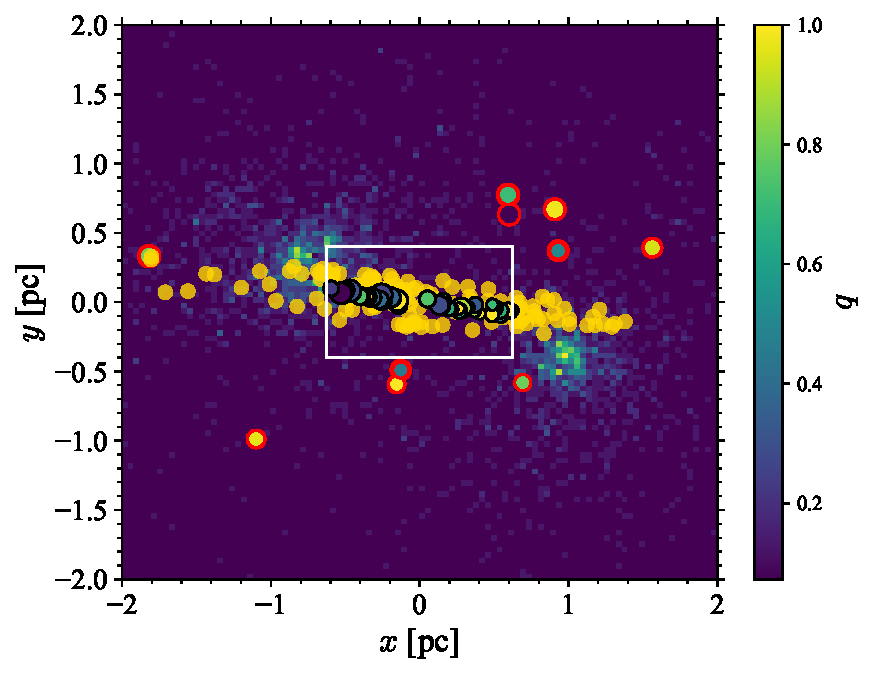
\includegraphics[width=\columnwidth]{figures/overplotting_HEATMAP.pdf}
        \caption{Schematic of a F05 simulation. The density map denotes final positions of simulated objects, the translucent yellow points observed stars taken from \citet{2016A&A...595A...1G, 2023A&A...674A...1G}. The white frame denotes the observed region in \citet{2023arXiv231001231P}, with black outlined dots denoting observed JuMBOs. Red outlined dots denote the final JuMBOs observed in our simulation.}
         \label{Fig:Overplot}
   \end{figure}

    Figure \ref{Fig:Overplot} shows the final snapshot of a F05 simulation. It represents the typical final state of simulations evolved during our $\mathcal{ISF}$ and $\mathcal{FFC}$ runs. The density map reveals the final positions of all objects simulated. Surviving JuMBOs are scattered onto the plot with red outlines. Overlayed are also the positions of known stars (in yellow) taken from \citet{2016A&A...595A...1G, 2023A&A...674A...1G} and the positions of known JuMBOs (black outlined points) \citep{2023arXiv231001231P}.

    Table \ref{Tab:Final_ISF_FFC_Results} summarises all our final results. We begin our discussion on the $\mathcal{ISF}$ models by looking at the general models (top segment of table \ref{Tab:ISF_FFC_Initial}). 
     
    \subsubsection{Open Parameter Space}
    Overall, JuMBOs are more likely to survive in a Plummer-like cluster. Their survival rates increase by a factor of $\sim 18$ compared with likewise configurations initialised under a Fractal distribution. Even so, no configuration is successful in reproducing the $9\%$ fraction of JuMBOs relative to free-floaters observed. Instead, in the $\mathcal{ISF}$ scenarios, the fraction of JuMBOs to JMO free floaters ranges between $0.29\sim1.3$ for Plummer runs and $0.01\sim0.02$ for Fractals.
    
    The increase of JuMBO surviveability in runs including free-floaters could be due to the rare JMO-JuMBO interaction hardening the binary, also resulting in a decrease in its gravitational cross section. We believe this to be the case even though as discussed in the introduction JuMBOs will tend to ionise, even when interacting with other JMO, since, although increasing the number of JMOs enhances the chances of two free-floaters (or a free floater and ionised JMO) settling into a newly formed binary, on average, only $0.4$ new JuMBO systems emerge per run for F05 runs compared to the $0.65$ in F05FF (from $1.75$ to $3.15$ between P05 and P05FF). 
    
    Figures \ref{Fig:Gen_Semi_Fractal} show the cumulative distribution function (CDF) for the semi-major axis of surviving JuMBOs during F05, F05FF and F1 runs. The Fractal distribution efficiently prunes off any wide orbits since its violent nature provokes many encounters result in the ionisation of JuMBO systems, moreso the ones on wide orbits who have a larger cross-section. The tendency for JuMBOs to ionise at any encounter is reflected by the little variation between runs of the same virial radius. We also note the tendency for JuMBOs to ionise even when a JMO perturbs the system as reflected with the decrease in median semi-major axis between models P05 and P05FF from $\langle a\rangle\sim268$ au to $\langle a\rangle\sim187$ au.
   
   \begin{figure}
    \centering
        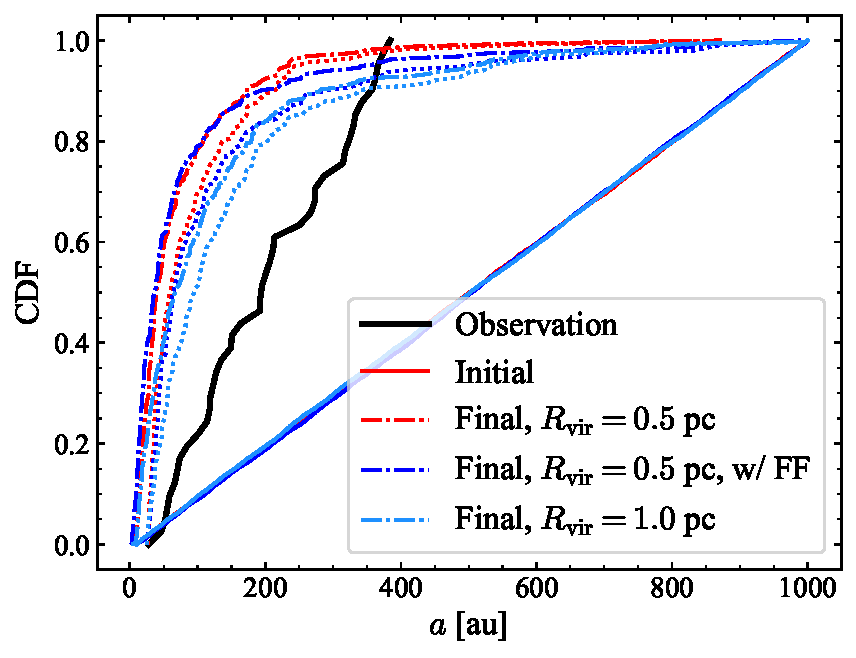
\includegraphics[width=\columnwidth]{figures/Fractal_General_sem_axis.pdf}
        \caption{CDF of surviving JuMBO semi-major axis distribution for models F05, F05FF, F1. Dash-dotted curves incorporate all JuMBO systems, whereas dotted ones only those with a projected separation exceeding $25$ au.}
         \label{Fig:Gen_Semi_Fractal}
   \end{figure}
    
    The results in semi-major axis' during the Fractal runs are much smaller than those observed, suggesting the $\mathcal{ISF}$ model fails to capture the birth of such environments. Contrariwise, and as seen in figure \ref{Fig:Gen_Semi_Plummer}, Plummer models are capable of preserving the wider orbits. This, however, is due to the environment to output similar values to those inputted since it is less violent by nature.
   
   \begin{figure}
    \centering
        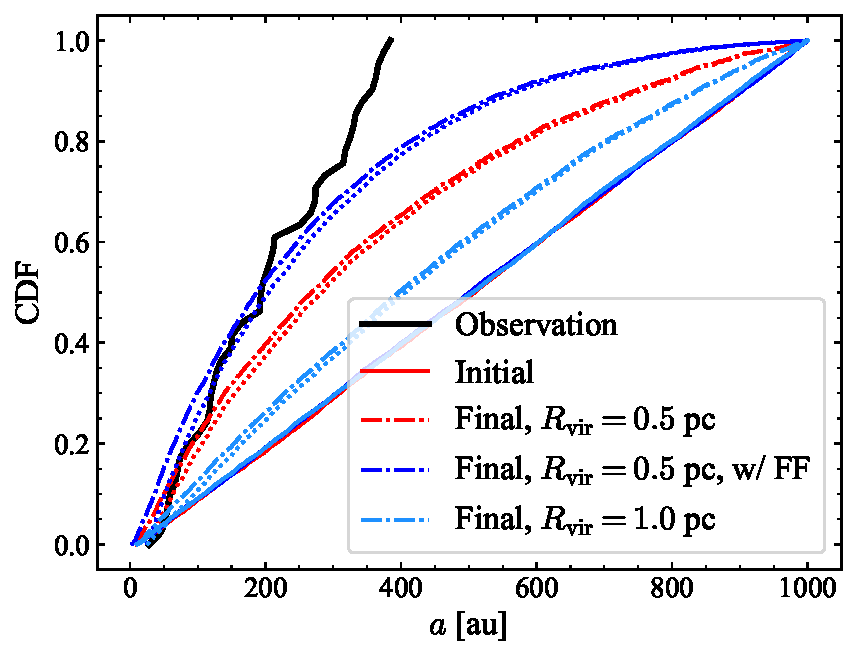
\includegraphics[width=\columnwidth]{figures/Plummer_General_sem_axis.pdf}
        \caption{CDF of surviving JuMBO semi-major axis distribution for models P05, P05FF, P1. Dash-dotted curves incorporate all JuMBO systems, whereas dotted ones only those with a projected separation exceeding $25$ au.}
         \label{Fig:Gen_Semi_Plummer}
   \end{figure}

    Indeed, keeping in mind that our JuMBOs in these models are initialised with a uniform mass distribution, we see the uniformity reflected in the final $M_{\mathrm{prim}}$ vs. $q$ parameter space shown in figure \ref{Fig:Gen_mdistr_Plummer}. Although it also fails at reproducing observations, figure \ref{Fig:Gen_mdistr_Fractal} shows more structure and less uniformity in the distribution of JuMBOs in ($M_{\mathrm{prim}}$, $q$)-space as reflected by the starker contrasts between contour levels and smaller high-density regions.
    
    Given this, although a correct calibration of initial conditions during Plummer runs will give back JuMBOs with similar properties to those observed, the extent of fine tuning needed and lack of natural mechanism to remove the tail end of wide-orbit JuMBOs, we can apply Occam's razor to rule it out as an initial conditions. 
    
    The omission of Plummer models is further supported since no systems formed dynamically during the runs. This contradicts with the observed presence of two triple JMO systems. Given this, we restrict ourselves to Fractal models as we believe this better represents the Trapezium cluster, a fact agreeing with \citet{2016MNRAS.457..313P}.
   
   \begin{figure}
    \centering
        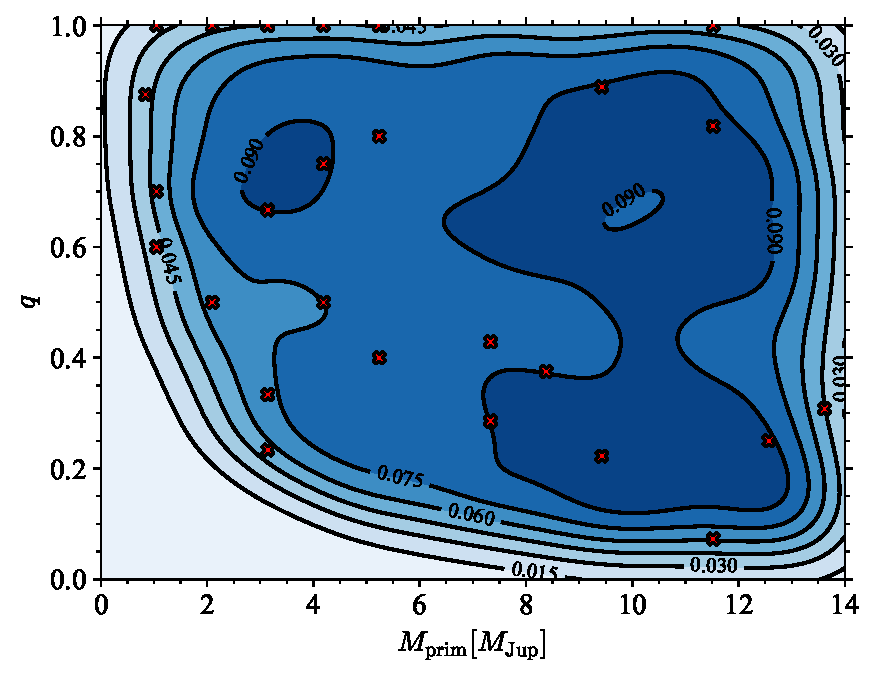
\includegraphics[width=\columnwidth]{figures/Plummer_rvir0.5_FF_mass_distr.pdf}
        \caption{Contour plot of $M_{\mathrm{prim}}$ vs. $q$ for model P05FF. Red crosses denote where observed JuMBOs lie.}
         \label{Fig:Gen_mdistr_Plummer}
   \end{figure}
   
   \begin{figure}
    \centering
        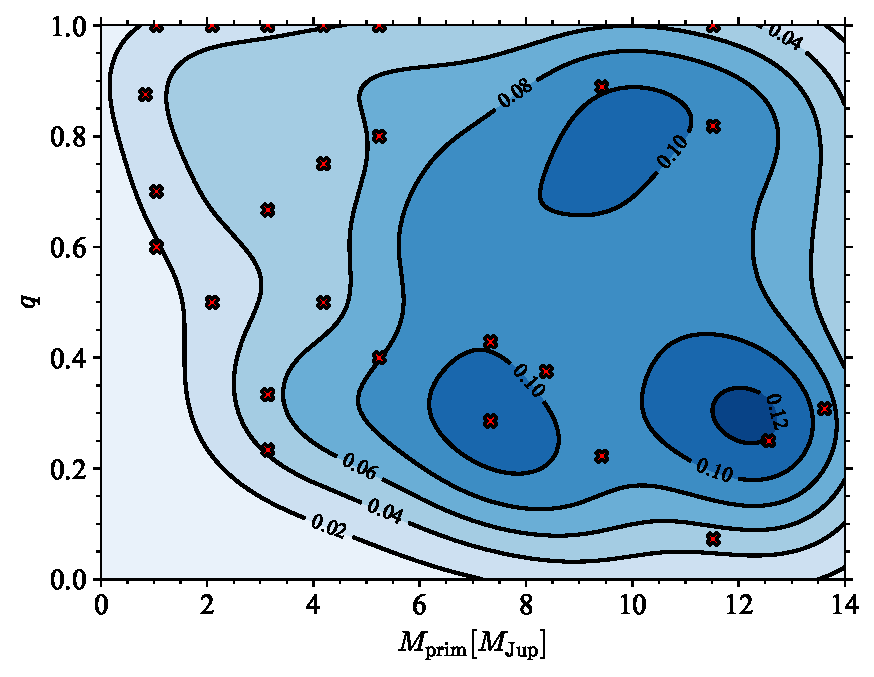
\includegraphics[width=\columnwidth]{figures/Fractal_rvir0.5_FF_mass_distr.pdf}
        \caption{Contour plot of $M_{\mathrm{prim}}$ vs. $q$ for model F05FF. Red crosses denote where observed JuMBOs lie.}
         \label{Fig:Gen_mdistr_Fractal}
   \end{figure}

    \subsubsection{Evolving till $10$ Myr: TO CHECK -- STILL IN RUNS}
        Here we analyse results for a system evolved to $10$ Myr, with the aim of looking at the survival of JuMBOs in more established systems. Overall, the JuMBO survival rate decreases and the ones surviving exhibit tighter orbits with $\langle a\rangle \sim 20$, a regime in which two $3\ M_{\mathrm{Jup}}$ systems become hard for $\sim M_{\mathrm{Jup}}$ interactions. 
        
        Figure \ref{Fig:Mdistr_SimTime} shows the distribution of $M_{\mathrm{prim}}$ of surviving JuMBOs. The little difference  observed between F05FF and F05FFL is reflected by the similarities between their median and interquartile (IQR) range ($\langle M_{\mathrm{prim}}\rangle\sim 8.8$ and $\langle M_{\mathrm{prim}}\rangle \sim 8.1$ for F05FF and F05FFL respectively). The fact that this holds for all configurations simulated implies the ease at which JuMBO systems ionise upon interaction.

        Figure \ref{Fig:SimTime_MPrimQ} shows the contour plot of $M_{\mathrm{prim}}$ vs. $q$. As before, the parameter space poorly replicates the observed distribution with most of the JuMBOs having too large a primary mass. We keep this in mind for simulations in the following subsection where we initialise JuMBOs with a power-law of $\alpha = -1.2$, the power-law found to best fit observations.
   
   \begin{figure}
    \centering
        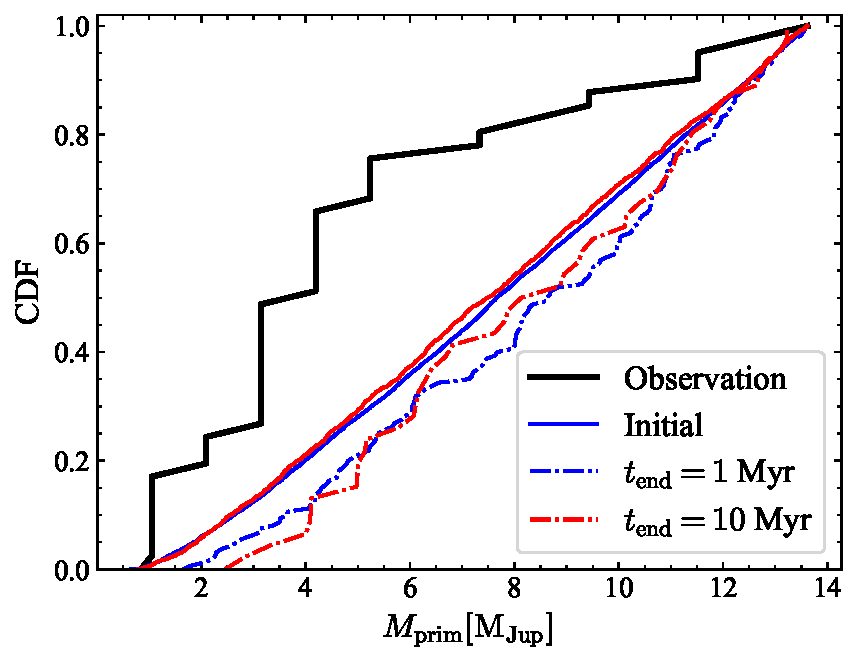
\includegraphics[width=\columnwidth]{figures/SimTime_mprim_vs_obs_.pdf}
        \caption{CDF of surviving JuMBO $M_{\mathrm{prim}}$ for models F05FF and F05FFL.}
         \label{Fig:Mdistr_SimTime}
   \end{figure}
   
   \begin{figure}
    \centering
        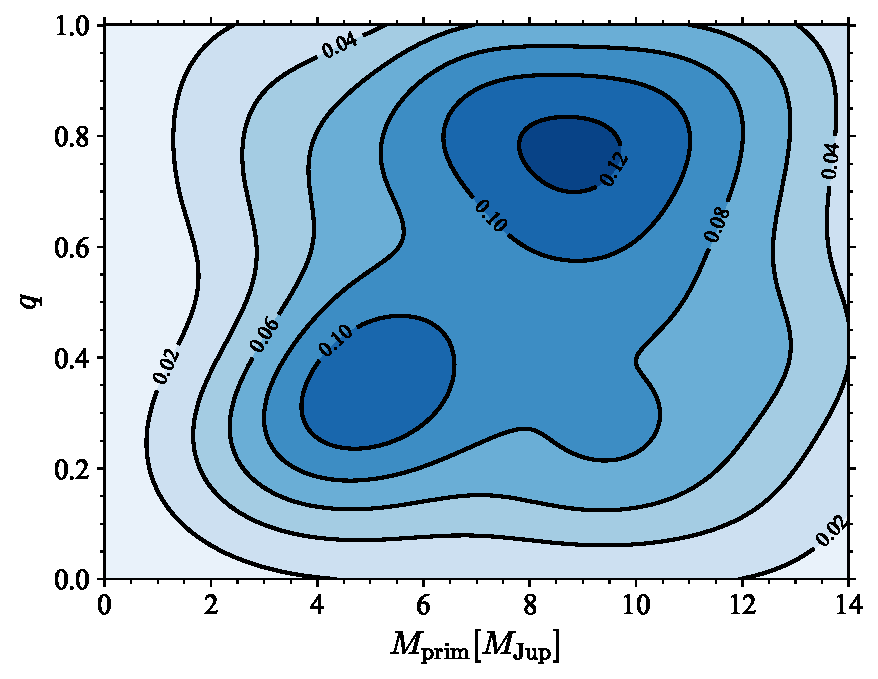
\includegraphics[width=\columnwidth]{figures/Fractal_rvir0.5_FF_10Myr_mass_distr.pdf}
        \caption{$M_{\mathrm{prim}}$ vs. $q$ contour plot for model F05FFL. Red crosses denote where observed JuMBOs lie.}
         \label{Fig:SimTime_MPrimQ}
   \end{figure}
   
    \subsubsection{Observational Constraints}
    Our preliminary exploration allows us to rule out Plummer models and further constrain the parameter space. When applying these more restricted initial conditions, $f_{\mathrm{surv}}$ and $e$ barely changes while $a$ shows only marginal changes.

    This slight increase in $f_{r_{ij}\geq25\ \mathrm{au}}$, $\langle a\rangle$ and $\langle r_{ij}\rangle$ could be attributed to the reduction of JMO and JuMBOs present in the environment and the smaller masses they occupy making it harder for them to destabilise wide binaries. The difference in the semi-major axis distribution between models F05, F05O and F05OC (JuMBOs are initially on circular orbits) is shown in figure \ref{Fig:Semi_Fractal}. No matter the configuration, the Fractal models exhibit a natural tendency for trimming out wide binaries.
    
   \begin{figure}
    \centering
        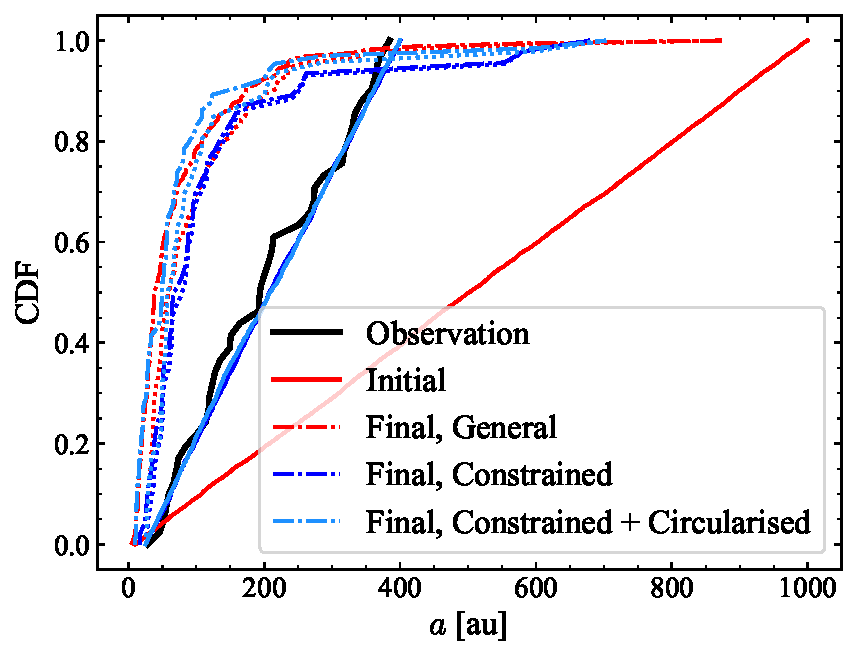
\includegraphics[width=\columnwidth]{figures/Fractal_noFF_sem_axis.pdf}
        \caption{CDF of surviving JuMBO semi-major axis distribution for models F05, F05O, F05OC.}
         \label{Fig:Semi_Fractal}
   \end{figure}

   Figure \ref{Fig:Fractal_mdistrCDF} shows the CDF of primary masses comparing models F05, F05O And F05OC. No matter the configuration, a similar evolution is observed where surviving JuMBOs tend to have larger primary masses. However, unlike the F05 model, the constrained model, initialised with $\alpha = -1.25$, end up being roughly uniform in primary mass compared to the somewhat thermal appearance for F05. In doing, the median primary masses shift towards lower values while the mass ratio towards larger one. A fact reflected by the statistics shown in table \ref{Tab:Final_ISF_FFC_Results} and shown in figure \ref{Fig:FractalObs_mdistr}.
    
   \begin{figure}
    \centering
        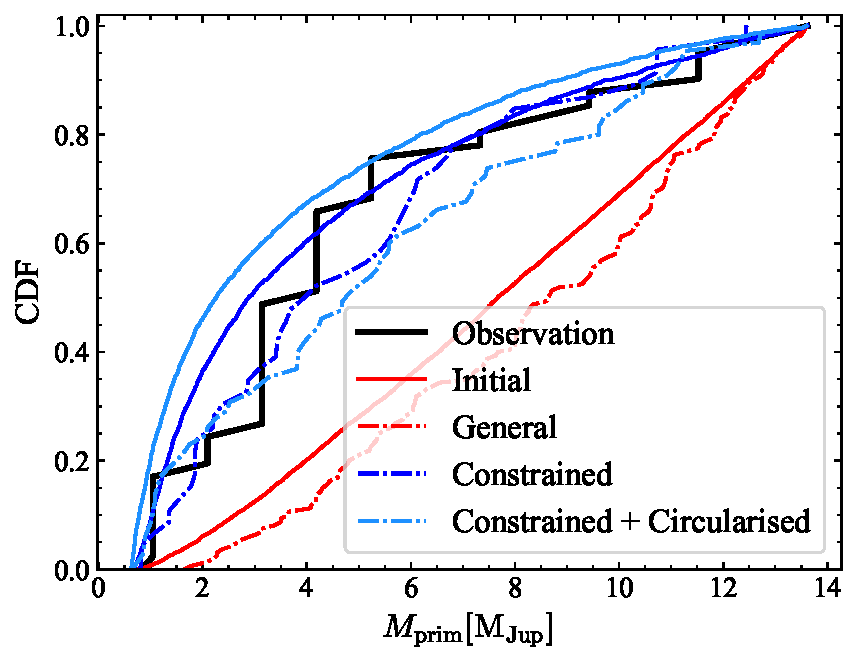
\includegraphics[width=\columnwidth]{figures/Fractal_noFF_mprim_vs_obs_.pdf}
        \caption{CDF of surviving JuMBO primary mass for models F05, F05O, F05OC.}
         \label{Fig:Fractal_mdistrCDF}
   \end{figure}

    Over the course of our simulation, Fractal runs exhibit a range of dynamical phenomena. The statistics of merging scenarios, and the emergence of both Jupier-mass - Stellar binary systems and $N\geq3$ systems are summarised in table \ref{Tab:Systems}.

    Jupiter-mass - stellar mergers could ................ In addition to mergers, ejection events also occured. Though no JuMBOs were ejected, $\sim1$ JMO was ejected per simulation and $\sim 3$ stellar-mass objects.
    
    Figure \ref{Fig:MixedSys_OrbParams} shows where in $(a,e)$-space Jupiter-mass - Stellar binaries lie, with little variation between configurations. The parameter space is widely covered, with signs of low-eccentricity but very wide ($a\geq700$ au) binaries. Nevertheless, the vast majority exhibit large eccentricities and semi-major axis, reflecting their dynamical origin. The non-negligible amount of these systems emerging provide an interesting prospect of detecting ultra-cold Jupiters orbiting stars who have recently fostered them.

    Given the poor reproducability in ratios of JuMBOs to JMO free floaters and the tight orbits of JuMBOs we conclude that the $\mathcal{ISF}$ models are most likely not the origins of JuMBOs, lending us to our final possible scenario, $\mathcal{FFC}$.

   \begin{figure}
    \centering
        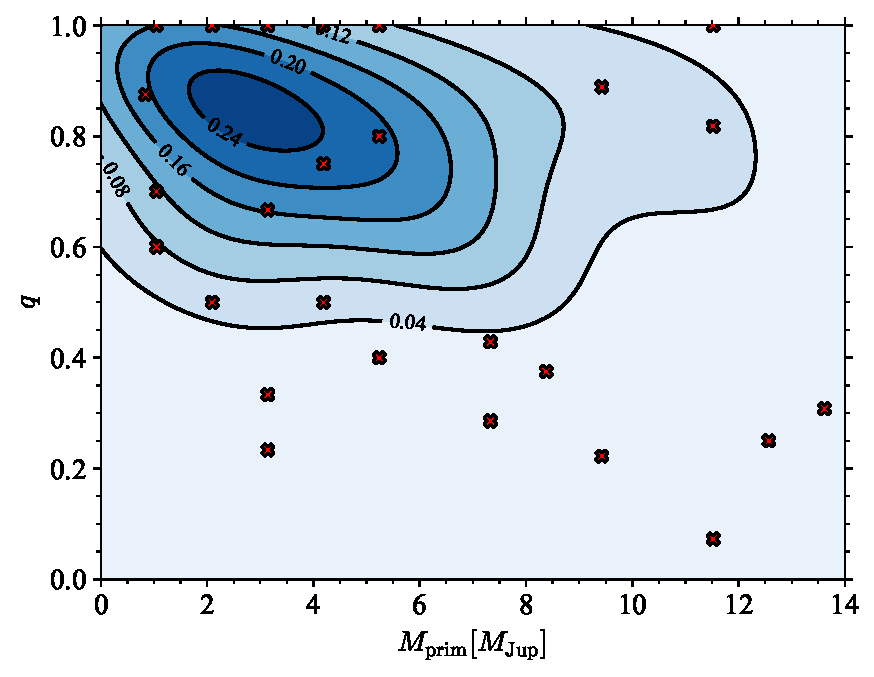
\includegraphics[width=\columnwidth]{figures/Fractal_rvir0.5_Obs_mass_distr.pdf}
        \caption{Contour plot of $M_{\mathrm{prim}}$ vs. $q$ for F05O. Red crosses denote where observed JuMBOs lie.}
         \label{Fig:FractalObs_mdistr}
   \end{figure}
   
   \begin{figure}
    \centering
        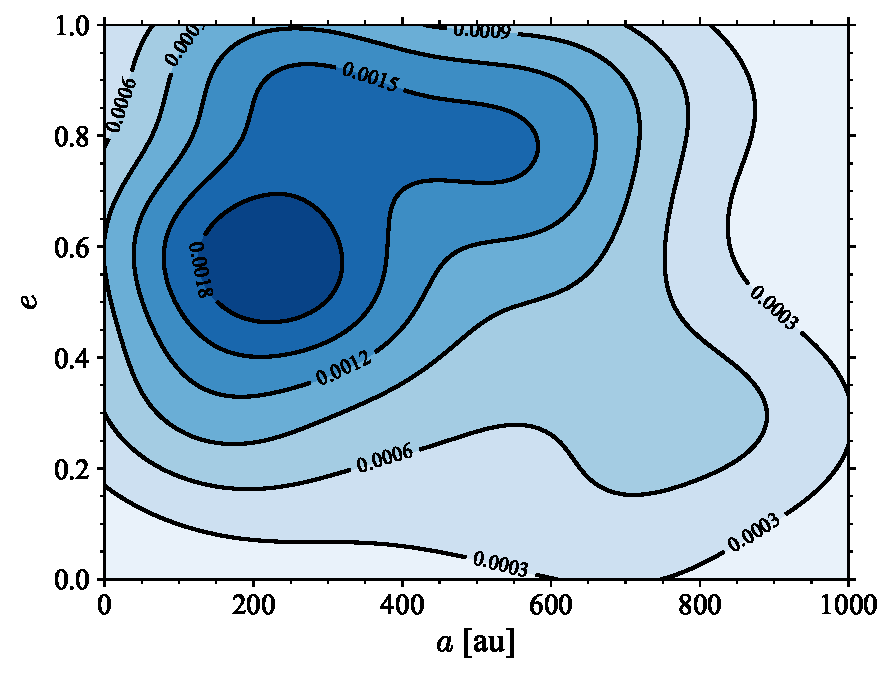
\includegraphics[width=\columnwidth]{figures/Fractal_rvir0.5_FF_Obs_sem_ecc_mixed_systs.pdf}
        \caption{$a$ vs. $e$ parameter space occupied by Star-JMO binaries during F05FFO runs.}
         \label{Fig:MixedSys_OrbParams}
   \end{figure}

    \begin{table}
         \caption{TO CHECK}
        \label{Tab:M2Events} 
        \centering 
        \begin{tabular}{c c c c c}
        \hline\hline
        Model & $\langle N_{\mathrm{JS, merge}}\rangle$ & $\langle N_{\mathrm{SS, merge}}\rangle$ & $\langle N_{\mathrm{JS}}\rangle$ &  $\langle N_{\mathrm{multi}} \rangle$ \\
        \hline \vspace{-0.75em}\\ 
           F05     & $2.5^{+0.5}_{-1.5}$ & $19^{+4}_{-7}$ & $8^{+3}_{-0}$  & $2^{+0}_{-0}$ \vspace{0.25em}\\
           F05FF   & $5.5^{+1.5}_{-1.5}$ & $21^{+2}_{-4}$ & $14^{+1}_{-3}$ & $2^{+0}_{-0}$ \vspace{0.25em}\\
           F1      & $1.0^{+1.0}_{-0.0}$ & $14^{+3}_{-5}$ & $10^{+1}_{-3}$ & $2^{+0}_{-0}$ \vspace{0.25em}\\
           F05FFL  & $5.0^{+0.0}_{-1.0}$ & $22^{+3}_{-5}$ & $1.0^{+0.0}_{-0.0}$ & $0^{+7}_{-0}$ \vspace{0.25em}\\
           \hline \vspace{-0.75em}\\
           F05O    & $2.0^{+0.8}_{-1.8}$ & $25^{+2}_{-8}$ & $4.5^{+2.8}_{-0.5}$ & $2.0^{+0}_{-0}$ \vspace{0.25em}\\
           F05FFO  & $1.0^{+1.0}_{-0.0}$ & $17^{+3}_{-1}$ & $5.0^{+1.5}_{-1.0}$ & $1.0^{+0}_{-0}$ \vspace{0.25em}\\
           F05OC   & $0.5^{+2.3}_{-0.5}$ & $20^{+5}_{-4}$ & $4.5^{+1.5}_{-1.5}$ & $3.5^{+0}_{-0}$ \vspace{0.25em}\\
           \hline
         \hline                               %inserts single line
         \label{Tab:Systems}
        \end{tabular}
     \end{table}
    \subsection{$\mathcal{FFC}$}
    

%--------------------------------------------------------------------
\section{Discussion}
 Lorem ipsum dolor sit amet, consectetur adipiscing elit, sed do eiusmod tempor incididunt ut labore et dolore magna aliqua. Ut enim ad minim veniam, quis nostrud exercitation ullamco laboris nisi ut aliquip ex ea commodo consequat. Duis aute irure dolor in reprehenderit in voluptate velit esse cillum dolore eu fugiat nulla pariatur. Excepteur sint occaecat cupidatat non proident, sunt in culpa qui officia deserunt mollit anim id est laborum.

%--------------------------------------------------------------------

\section{Conclusions}

\subsection{Energy Consumption}
The $820$ simulations conducted during this investigation had a total wall-clock time of $432$ days. For the XYZ runs, each CPU used $6$ cores, for the other two configurations $18$ cores were used per CPU. In total, the CPU time for all simulations was $7680$ days. Assuming a CPU consumption rate of $12$ Watt hr$^{-1}$ \citep{PortegiesZwart2020}, the total energy consumption is roughly $2210$ kWh. For an emission intensity of $0.283$ kWh kg$^{−1}$ \citep{Wittman}, our calculations emitted $7.8$ tonnes of CO2, roughly equivalent to two round trips by plane New York - Beijing.

\begin{acknowledgements}
Veronica  Saz  Ulibarrena,  Shuo  Huang,  Maite  Wilhelm,  Brent Maas
\end{acknowledgements}

% for the bibliography, at the end
\bibliographystyle{aa} % style aa.bst
\bibliography{references.bib} % your references Yourfile.bib

\begin{appendix}
    \section{Similarity between $r_{ij}$ and $a$}
    Figures \ref{Fig:Plummer_rsep} and \ref{Fig:Fractal_rsep} motivate our choice of analysing results in terms of the semi-major axis given the similarity between the curves. 
    
    In all cases, $r_{ij}$ exhibits longer tails at the detriment of the shorter separations/orbits. However, these differences are so small - especially in the Fractal case for which most of our discussion revolves around - that we can safely interchange between one and the other. In doing so, we assume that the observed projected separation of JuMBOs are equivalent to their semi-major axis, easing our discussion.
    
    \begin{figure}
    \centering
        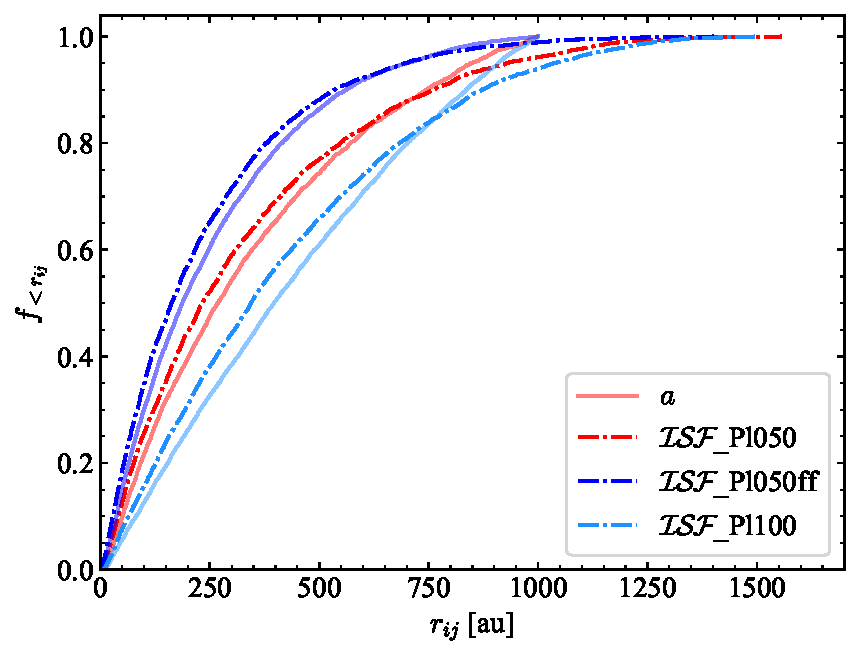
\includegraphics[width=\columnwidth]{figures/Plummer_General_proj_sep.pdf}
        \caption{CDF of surviving JuMBO projected separation distribution for models P05, P05FF, P1. Overplotted are translucent lines denoting the respective models' JuMBOs semi-major axis.}
         \label{Fig:Plummer_rsep}
   \end{figure}
   \begin{figure}
    \centering
        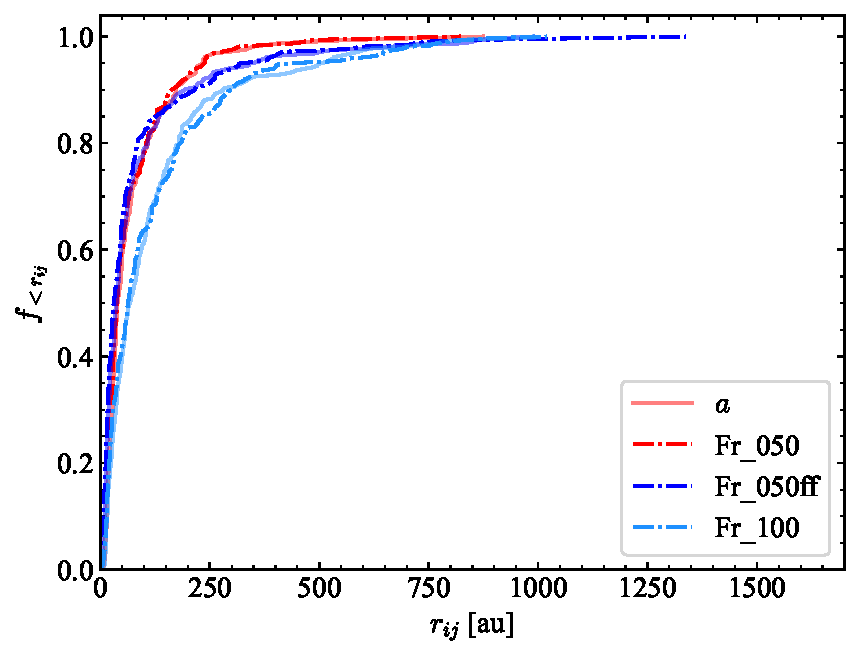
\includegraphics[width=\columnwidth]{figures/Fractal_General_proj_sep.pdf}
        \caption{CDF of surviving JuMBO projected separation distribution for models F05, F05FF, F1. Overplotted are translucent lines denoting the respective models' JuMBOs semi-major axis.}
         \label{Fig:Fractal_rsep}
   \end{figure}
\end{appendix}

\end{document}

%%%%%%%%%%%%%%%%%%%%%%%%%%%%%%%%%%%%%%%%%%%%%%%%%%%%%%%%%%%%%%
%-------------------------------------------------------------------
% END OF TEXT
%-------------------------------------------------------------------
%%%%%%%%%%%%%%%%%%%%%%%%%%%%%%%%%%%%%%%%%%%%%%%%%%%%%%%%%%%%%%

